\documentclass[12pt,a4paper]{article}

% --- Language and Encoding ---
\usepackage[utf8]{inputenc}
\usepackage[T1]{fontenc}
\usepackage[english,romanian]{babel}

% --- Layout and Graphics ---
\usepackage{geometry}
\geometry{left=2cm, right=2cm, top=2cm, bottom=2cm}
\usepackage{graphicx}
\usepackage{fancyhdr}
\usepackage{xcolor}

% --- Tables and Math ---
\usepackage{array}
\usepackage{booktabs}
\usepackage{amsmath}
\usepackage{amssymb}

% --- Code Listings ---
\usepackage{listings}
\usepackage{hyperref}
\hypersetup{
    colorlinks=true,
    linkcolor=black,
    urlcolor=blue
}

% --- Listings Configuration ---
\lstset{
    language=Python,
    basicstyle=\ttfamily\small,
    keywordstyle=\color{blue},
    commentstyle=\color{gray},
    stringstyle=\color{red},
    breaklines=true,
    tabsize=4,
    frame=single,
    backgroundcolor=\color{gray!10},
    inputencoding=utf8,
    extendedchars=true,
    literate={ă}{{\u{a}}}1 {â}{{\^{a}}}1 {î}{{\^{i}}}1 {ș}{{\c{s}}}1 {ț}{{\c{t}}}1
}

% --- Header and Footer ---
\pagestyle{fancy}
\fancyhf{}
\rhead{\thepage}
\lhead{Raport Temă Practică}

% --- Title Data ---
\title{\textbf{Raport Temă Practică ML}}
\author{Aldea Alexandra-Maria, Cotea Carla-Gabriela}
\date{Ianuarie 2026}

\begin{document}

\maketitle

\section{Preprocesare (Task 2.1)}

\subsection{Clasificarea Produselor}

\subsubsection*{Scop}

Primul pas a fost împărțirea produselor pe categorii generalizate din produsele particulare din datasetul original (de exemplu, \textit{``Pepsi''}, \textit{``Crazy Schnitzel''}, \textit{``French fries''}). De asemenea, s-au adăugat coloanele de \texttt{tip\_zi} (weekday/weekend) și \texttt{perioada\_zi} (morning/lunch/evening).

\subsubsection*{Implementare}

Scriptul \texttt{add\_category\_column.py} definește o funcție care primește numele produsului și, pe baza unor liste predefinite, atribuie o categorie.

\begin{lstlisting}
def categorize_product(product_name):
    if 'Pepsi' in product_name or 'Aqua' in product_name:
        return 'drink'
    elif product_name in ['Crazy Sauce', 'Cheddar Sauce', ...]:
        return 'sauce'
    elif 'Schnitzel' in product_name:
        return 'schnitzel'
    # ... etc
\end{lstlisting}

\subsubsection*{Categorii Definite}

Am împărțit toate produsele în 9 categorii semantice:

\begin{itemize}
    \item \textbf{drink}: Băuturi (Pepsi, Aqua, Lipton, etc.)
    \item \textbf{sauce}: Sosuri comandate standalone (Crazy Sauce, Cheddar Sauce, etc.)
    \item \textbf{schnitzel}: Schnitzele
    \item \textbf{side\_dish}: Garnituri (cartofi)
    \item \textbf{main\_dish}: Fel principal (Mac \& Cheese, Chicken Bao Buns)
    \item \textbf{extra}: Ingrediente extra
    \item \textbf{salad}: Salate
    \item \textbf{dessert}: Deserturi
    \item \textbf{packaging}: Ambalaj
\end{itemize}

\subsubsection*{Exemplu după categorizare}

\begin{table}[h]
    \centering
    \caption{Exemplu date după categorizare}
    \vspace{0.2cm}
    \begin{tabular}{lllll}
        \toprule
        \textbf{id\_bon} & \textbf{Product Name} & \textbf{Category} & \textbf{tip\_zi} & \textbf{perioada\_zi} \\
        \midrule
        1 & Crazy Schnitzel & schnitzel & weekday & lunch \\
        1 & Crazy Sauce & sauce & weekday & lunch \\
        1 & Pepsi & drink & weekday & lunch \\
        2 & Crazy Schnitzel & schnitzel & weekend & evening \\
        2 & French fries & side\_dish & weekend & evening \\
        \bottomrule
    \end{tabular}
\end{table}

\subsection{Agregare la Nivel de Bon}

\subsubsection*{Problema}

După pasul anterior, datele sunt la nivel de produs individual. Pentru a antrena un model de clasificare la nivel de bon, trebuie agregate informațiile tuturor produselor pe fiecare bon.

\subsubsection*{Transformarea Datelor}

Scriptul \texttt{create\_modified\_dataset.py} transformă datele prin:

\begin{enumerate}
    \item Grupare după \texttt{id\_bon}.
    \item Pentru fiecare bon, numărare a produselor per categorie.
    \item Pentru fiecare bon, numărare a fiecărui produs specific.
    \item Creare de coloane noi: \texttt{count\_category\_*} și \texttt{count\_product\_*}.
\end{enumerate}

\subsubsection*{Exemplu Transformare}

\textbf{ÎNAINTE} (nivel de produs):

\begin{table}[h]
\centering
\begin{tabular}{llc}
\toprule
\textbf{id\_bon} & \textbf{retail\_product\_name} & \textbf{product\_category} \\
\midrule
1 & Crazy Schnitzel & schnitzel \\
1 & Crazy Sauce & sauce \\
1 & Pepsi & drink \\
2 & Crazy Schnitzel & schnitzel \\
2 & French fries & side\_dish \\
\bottomrule
\end{tabular}
\end{table}

\vspace{0.5cm}

\textbf{DUPĂ} (nivel de bon):

\begin{table}[h]
\centering
\begin{tabular}{ccccc}
\toprule
\textbf{id\_bon} & \textbf{count\_cat\_schnitzel} & \textbf{count\_cat\_sauce} & \textbf{count\_prod\_sauce} & $\ldots$ \\
\midrule
1 & 1 & 1 & 1 & \\
2 & 1 & 0 & 0 & \\
\bottomrule
\end{tabular}
\end{table}

\subsection{Filtrare și Extragere Features Finale}

\subsubsection*{Context}

Scriptul \texttt{filter\_crazy\_schnitzel+features.py} realizează următoarele:

\begin{enumerate}
    \item Filtrează doar bonuri care conțin \textit{Crazy Schnitzel}.
    \item Creează eticheta target.
    \item Computează caracteristici de coș.
\end{enumerate}

\subsubsection*{1. Filtrare Inițială}

\begin{lstlisting}
bonuri_cu_crazy_schnitzel = df[df['retail_product_name'] == 'Crazy Schnitzel']['id_bon'].unique()
df = df[df['id_bon'].isin(bonuri_cu_crazy_schnitzel)]
\end{lstlisting}

\subsubsection*{2. Eticheta Target (\texttt{y})}

\begin{lstlisting}
bonuri_cu_crazy_sauce = df[df['retail_product_name'] == 'Crazy Sauce']['id_bon'].unique()
df['y'] = df['id_bon'].apply(lambda x: 1 if x in bonuri_cu_crazy_sauce else 0)
\end{lstlisting}

Variabila target este binară:

\begin{itemize}
    \item $y = 1$: Bonul conține \textit{Crazy Sauce}.
    \item $y = 0$: Bonul NU conține \textit{Crazy Sauce}.
\end{itemize}

\subsubsection*{3. Caracteristici de Coș}

Pentru fiecare bon, calculez caracteristici agregate:

\begin{table}[h]
\centering
\caption{Caracteristici de coș}
\vspace{0.2cm}
\begin{tabular}{ll}
\toprule
\textbf{Feature} & \textbf{Descriere} \\
\midrule
\texttt{cart\_size} & Numărul total de produse pe bon \\
\texttt{distinct\_products} & Numărul de produse DIFERITE comandate \\
\texttt{total\_value} & Valoarea totală a comenzii (în bani) \\
\texttt{avg\_price} & Preț mediu per produs \\
\texttt{count\_category\_*} & Numărul de produse din fiecare categorie \\
\bottomrule
\end{tabular}
\end{table}

\section*{Rezumat Complet al Fluxului}

\[
\begin{array}{c}
\text{\texttt{dataset-original.csv}} \\
\text{(15000+ linii, nivel de produs)} \\
\downarrow \\
\boxed{\text{add\_category\_column.py}} \\
\text{Adaugă categorie, features temporale} \\
\downarrow \\
\text{\texttt{dataset-modified.csv}} \\
\text{(15000+ linii + categorie)} \\
\downarrow \\
\boxed{\text{create\_modified\_dataset.py}} \\
\text{Agregare pe bon, numărare per categorie și produs} \\
\downarrow \\
\text{\texttt{dataset-modified-features.csv}} \\
\text{(~4000 linii - bonuri, ~50 coloane - count\_*)} \\
\downarrow \\
\boxed{\text{filter\_crazy\_schnitzel+features.py}} \\
\text{Filtrare, creare y, features coș} \\
\downarrow \\
\text{\texttt{dataset-bon-features.csv}} \\
\textbf{FINAL: Gata pentru antrenare}
\end{array}
\]

\section{Preprocesare (Task 2.2)}

Același flux de preprocesare a fost aplicat și pentru problema 2.2. Diferența majoră a constat în absența etapei de filtrare, utilizându-se toate bonurile disponibile, nu doar cele care conțineau produsul \textit{Crazy Schnitzel}. Variabila țintă ($y$) a fost, pe rând, fiecare dintre cele 8 sosuri posibile, la antrenare acesta fiind exclus din trăsăturile furnizate pentru a evita ``scurgerile de date'' (\textit{data leakage}).

\section{Regresie Logistică (Task 2.1)}

Această secțiune detaliază procesul iterativ prin care am optimizat implementarea proprie a Regresiei Logistice, deciziile luate privind preprocesarea datelor și selecția hiperparametrilor, precum și comparația finală cu implementarea de referință din \texttt{scikit-learn}.

\subsection{Implementare finală}

Pentru rezolvarea problemei de clasificare binară (predicția sosului \textit{Crazy Sauce}), a fost implementată Regresia Logistică folosind metoda Gradient Descent cu optimizator Adam cu un $\alpha = 0.01$.
Minimizarea erorii s-a realizat folosind funcția de cost Binary Cross-Entropy, aceasta fiind standardul pentru problemele de clasificare binară. 

În varianta finală, am implementat mecanismul de regularizare L2 pentru a penaliza ponderile excesive și a evita overfitting-ul. A fost inclus și un mecanism de early stopping setat să se declanșeze după 10 epoci consecutive în care funcția de loss crește.

Un aspect crucial pentru eficiența algoritmului de optimizare a fost preprocesarea datelor prin standardizare. Am transformat variabilele de intrare astfel încât să aibă media 0 și deviația standard 1. 

Nu în ultimul rând, stabilitatea numerică la începutul antrenării a fost asigurată prin inițializarea ponderilor folosind metoda Xavier, prevenind astfel saturația prematură a funcției de activare Sigmoid.

\subsection{Evoluția experimentului}

Performanța modelului a fost obținută printr-un proces iterativ de optimizare, rezultatele fiind monitorizate constant comparativ cu baseline-ul \texttt{sklearn}.

\subsubsection*{Experimente cu SGD fără optimizator}

În prima fază a experimentelor, am rulat modelul pe datele brute cu regularizare L2 și un $lr=0.1$. Această abordare a rezultat într-o acuratețe modestă de aproximativ $65.83\%$, sub-performând masiv față de implementarea de referință ($76.47\%$). Diferența de peste $10\%$ a indicat clar că datele necesită o scalare corespunzătoare.

Un salt major a fost realizat prin adăugarea de trăsături de tip contor (\textit{counter features}). Maparea produselor specifice și generarea unor contoare per categorie au permis modelului să generalizeze comportamentul clienților. Această modificare a propulsat acuratețea la aproximativ $87\%$, după normalizarea datelor ajungând ulterior la $96.64\%$.

Ulterior, am setat o rată de învățare agresivă ($learning\_rate = 0.3$) combinată cu mecanismul de Early Stopping (patience = 5 epoci), însă, în mod surprinzător, acesta nu a fost declanșat pe parcursul experimentelor. 

Diferența critică a fost făcută de numărul de iterații. Rularea pentru 10.000 de iterații a adus modelul la paritate cu \texttt{sklearn} ($99.16\%$), iar extinderea la 15.000 de iterații a permis depășirea baseline-ului pe metricile punctuale, atingând o acuratețe de $99.44\%$.

Am mai experimentat și testând limitele absolute ale implementării prin rularea a 50.000 de iterații, am reușit să minimizez funcția de loss până la valoarea de $0.0160$, și se putea observa de pe plot-ul funcției de loss că aceasta încă scădea.

Este important de menționat și un experiment care nu a dat rezultatele așteptate: implementarea unui \textit{Learning Rate Decay}. Scăderea treptată a ratei de învățare a degradat performanța la nivelul etapelor intermediare (Acc $\approx 98.32\%$), deoarece rata scădea prea rapid, împiedicând modelul să parcurgă pașii necesari pentru a ajunge în zona de minim global atinsă anterior cu rata constantă.

\subsubsection*{Experimente cu Optimizator Adam}

Deoarece rata de învățare din experimentele anterioare era foarte agresivă, iar \textit{learning rate decay}-ul nu a funcționat la înălțimea așteptărilor, am integrat un optimizator \textbf{Adam} (Adaptive Moment Estimation) și am modificat patience = 10 în cadrul mecanismului de Early Stopping.

Parametrii utilizați pentru Adam au fost:
\begin{itemize}
    \item \textbf{Learning Rate}: $\alpha = 0.01$.
    \item \textbf{Exponential Decay Rates}: $\beta_1 = 0.9$, $\beta_2 = 0.999$.
    \item \textbf{Epsilon}: $\epsilon = 10^{-8}$.
\end{itemize}

Utilizarea optimizatorului Adam a schimbat radical dinamica antrenării. Deși acuratețea finală a rămas similară cu cea mai bună variantă SGD ($99.44\%$), \textbf{viteza de convergență a crescut semnificativ}. 

Dacă metoda SGD necesita 15.000 de iterații pentru a stabiliza funcția de cost în jurul valorii de $0.0022$, optimizatorul Adam a atins același prag de eroare și performanță în aproximativ \textbf{3.500 de iterații}. Acest lucru demonstrează eficiența superioară a gradientului adaptiv în navigarea suprafeței de eroare, eliminând necesitatea setării manuale a unei rate de învățare riscante.

\begin{table}[h]
    \centering
    \caption{Performanța Finală: Implementare Proprie vs. Scikit-Learn}
    \vspace{0.2cm}
    \begin{tabular}{lccc}
        \toprule
        \textbf{Metrică} & \textbf{Custom Implementation} & \textbf{sklearn} & \textbf{Diferență} \\
        \midrule
        Accuracy & 0.9944 & 0.9916 & +0.0028 \\
        Precision & 0.9896 & 0.9895 & +0.0001 \\
        Recall & 1.0000 & 0.9947 & +0.0053 \\
        F1-Score & 0.9948 & 0.9921 & +0.0027 \\
        ROC-AUC & 0.9996 & 0.9995 & +0.0001 \\
        \bottomrule
    \end{tabular}
\end{table}
 \newpage


\subsection{Matricea de Confuzie}

Pentru a vizualiza performanța modelului pe setul de testare, am generat matricea de confuzie (Figura \ref{fig:conf_matrix}). Aceasta ilustrează capacitatea modelului de a distinge corect între bonurile care conțin \textit{Crazy Sauce} și cele care nu.

\begin{figure}[h]
    \centering
    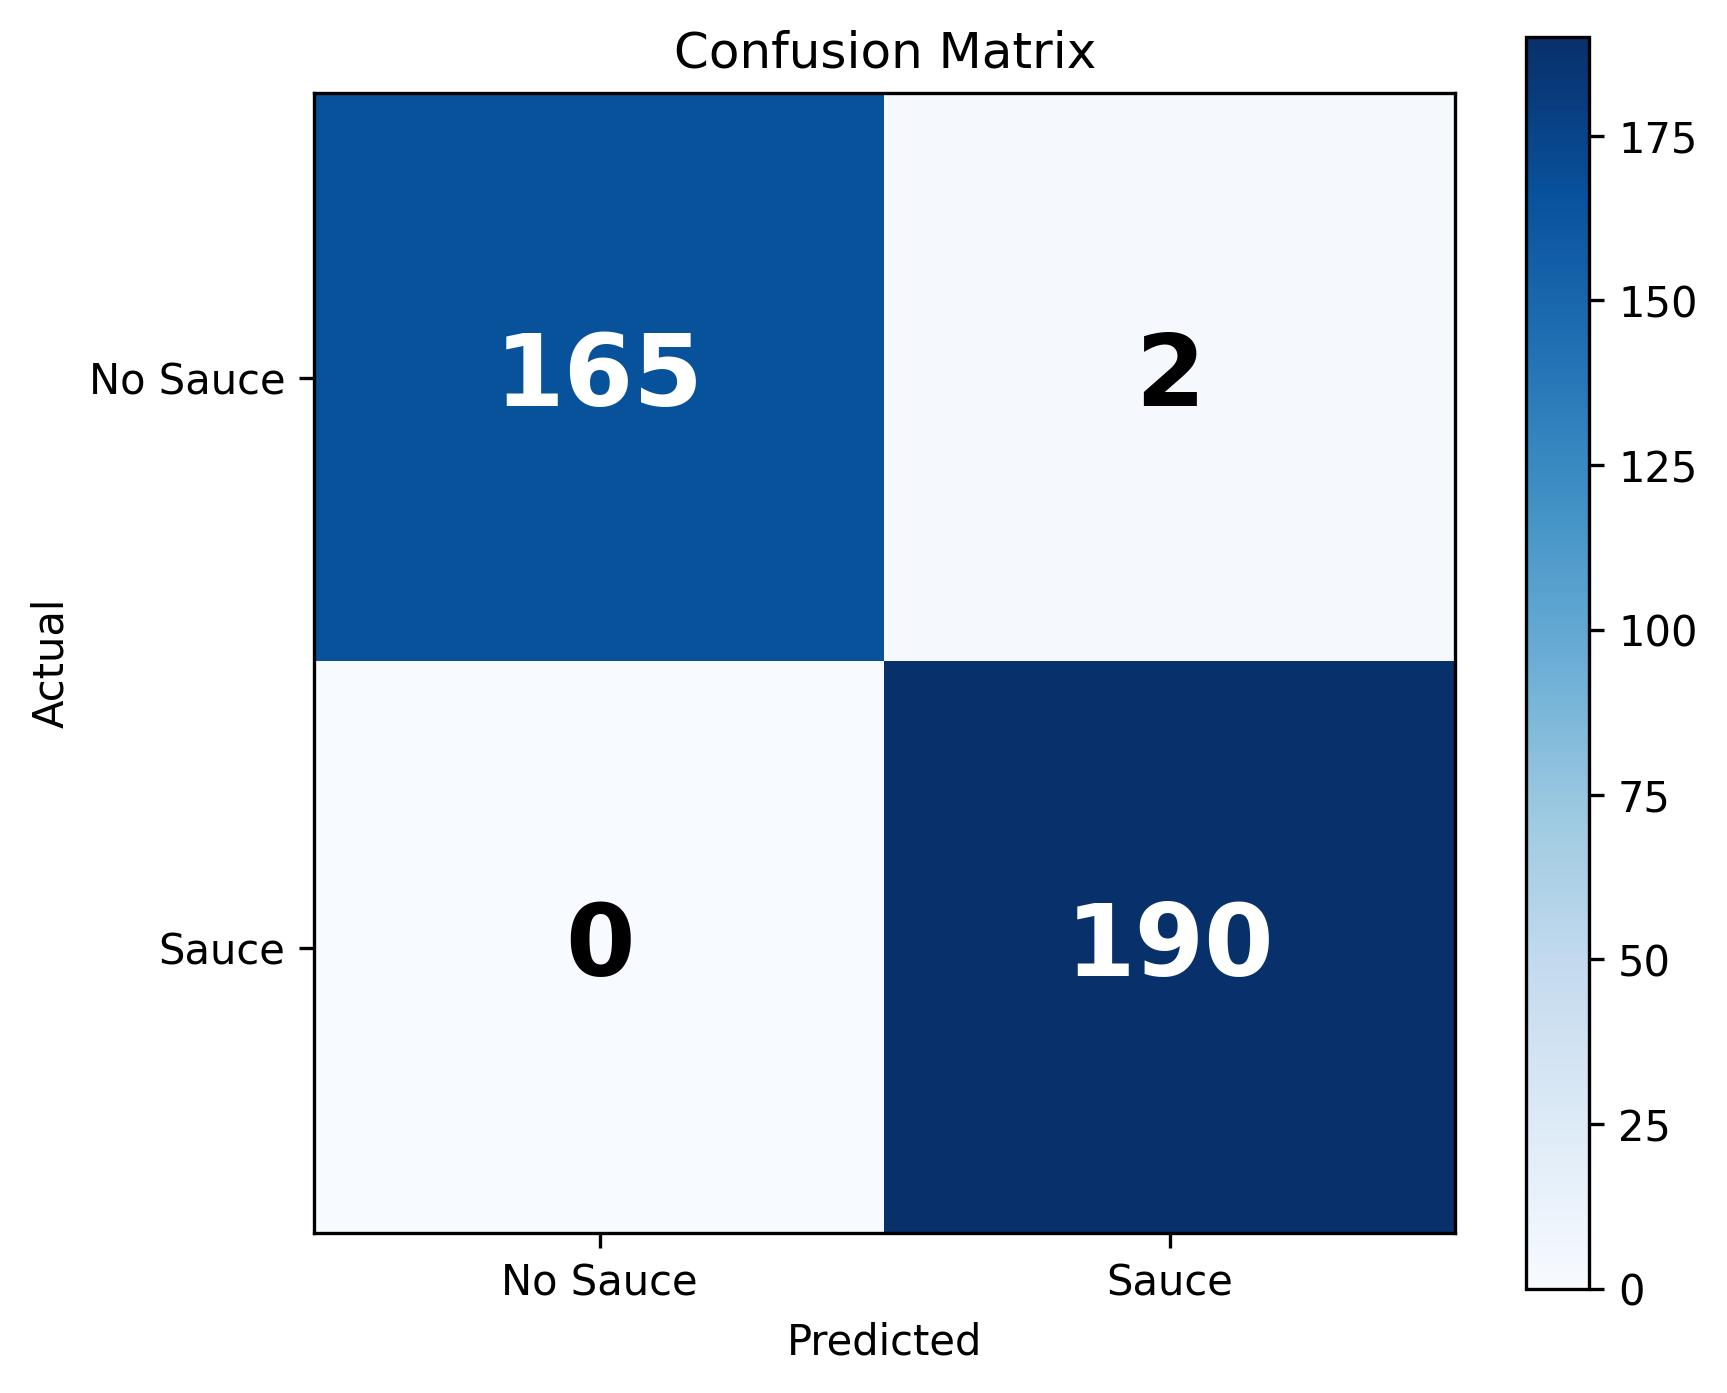
\includegraphics[width=0.6\textwidth]{confusion_matrix.jpg} 
    \caption{Matricea de Confuzie pentru clasificarea binară a sosului Crazy Sauce.}
    \label{fig:conf_matrix}
\end{figure}

Rezultatele indică o precizie extrem de ridicată:
\begin{itemize}
    \item \textbf{True Negatives (TN):} 165 (Bonuri fără sos clasificate corect)
    \item \textbf{True Positives (TP):} 190 (Bonuri cu sos clasificate corect)
    \item \textbf{False Positives (FP):} 2 (Bonuri fără sos clasificate greșit ca având sos)
    \item \textbf{False Negatives (FN):} 0 (Niciun bon cu sos nu a fost ratat)
\end{itemize}

\subsection{Analiza Curbei ROC}

Graficul demonstrează o capacitate de discriminare aproape ideală pentru ambele modele, curbele tinzând rapid către colțul stânga-sus (Rata de Pozitive Adevărate = 1, Rata de Pozitive False = 0).praguri de discriminare (Figura \ref{fig:roc_curve}).
\begin{figure}[h]
    \centering
    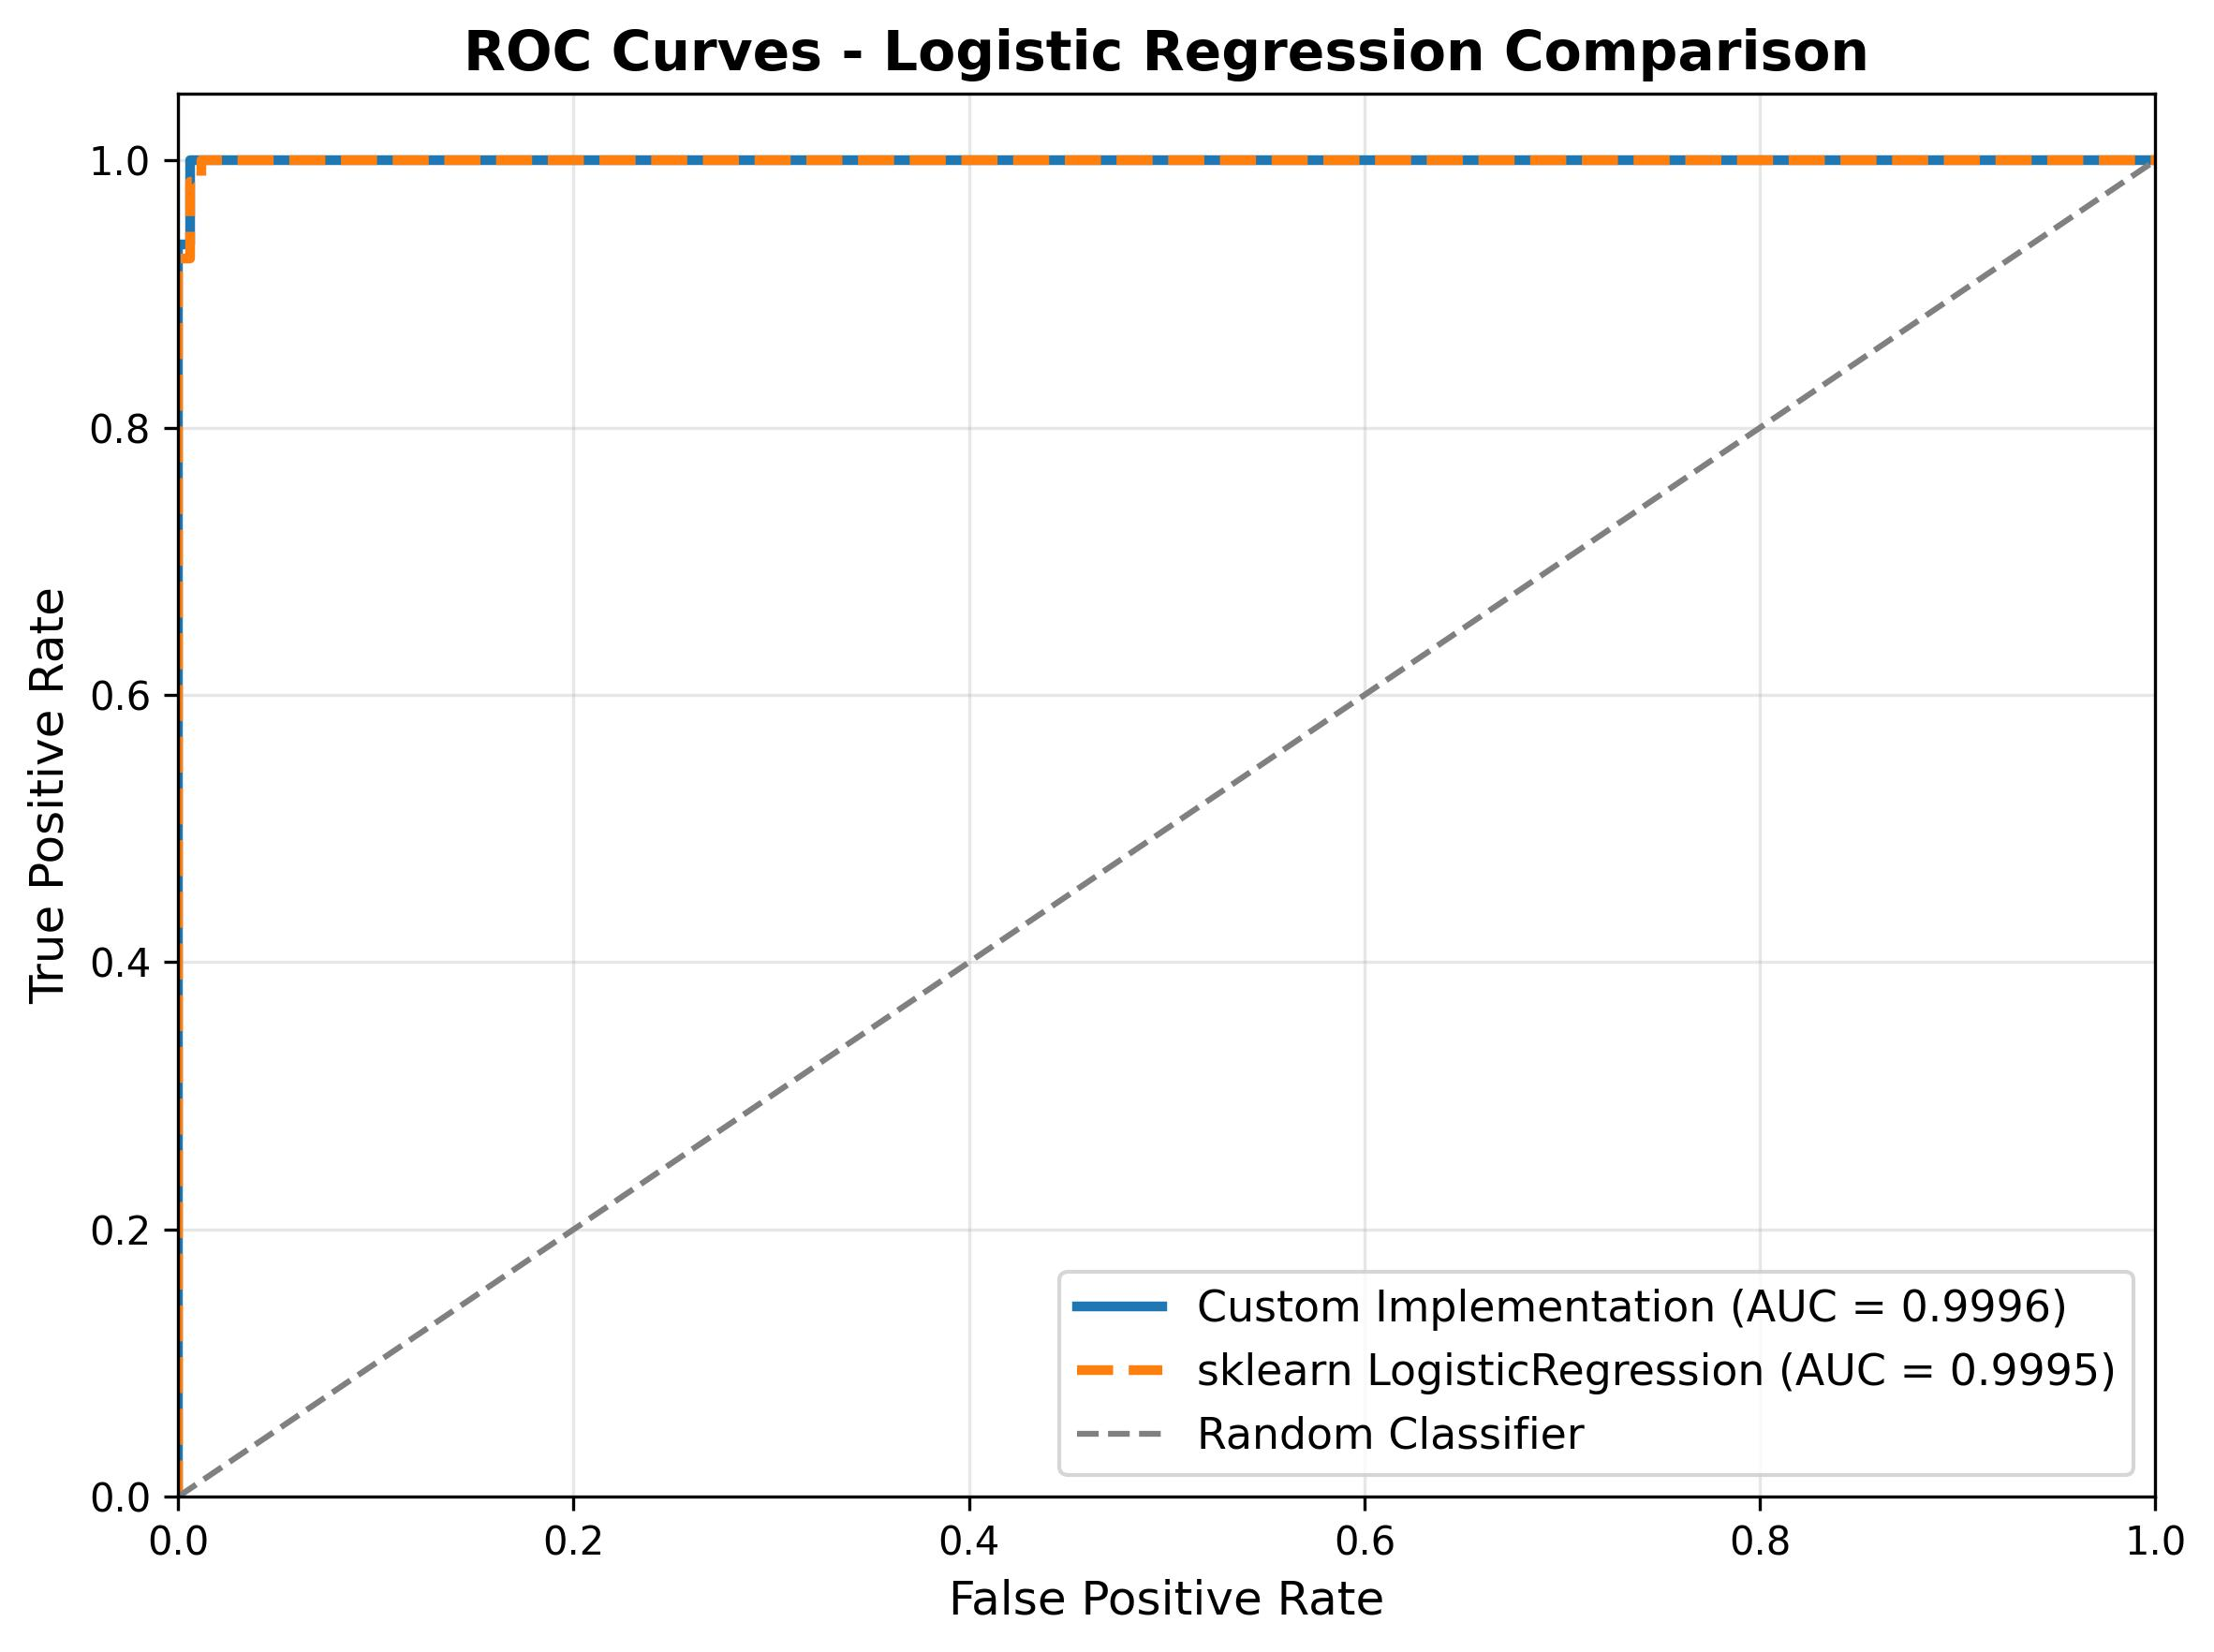
\includegraphics[width=0.6\textwidth]{roc_curve.jpg}
    \caption{Comparație curbe ROC: Implementare Proprie vs. Scikit-Learn.}
    \label{fig:roc_curve}
\end{figure}

\newpage

\subsection{Interpretarea Coeficienților Regresiei Logistice}

Un avantaj major al Regresiei Logistice este interpretabilitatea. Analizând ponderile ($w$) asociate fiecărei trăsături, putem înțelege ce factori influențează decizia clientului de a cumpăra \textit{Crazy Sauce}.

\subsubsection*{Factori care CRESC probabilitatea de cumpărare (Coeficienți Pozitivi)}
\begin{itemize}
    \item \textbf{Mărimea Coșului (\texttt{cart\_size}, $+12.04$):} Acesta este de departe cel mai puternic predictor. Cu cât un client comandă mai multe produse, cu atât este mai probabil să comande și un sos.
    \item \textbf{Valoarea Totală (\texttt{total\_value}, $+3.97$):} Corelat cu mărimea coșului, clienții care cheltuie mai mult sunt mai dispuși să adauge produse complementare.
    \item \textbf{Diversitatea (\texttt{distinct\_products}, $+1.98$):} O varietate mai mare de produse în coș indică o masă complexă, care necesită adesea sosuri.
\end{itemize}

\subsubsection*{Factori care SCAD probabilitatea de cumpărare (Coeficienți Negativi)}
\begin{itemize}
    \item \textbf{Alte Sosuri (\texttt{has\_cheddar\_sauce}, $-4.91$; \texttt{has\_garlic\_sauce}, $-4.19$):} Dacă un client a comandat deja un alt tip de sos, probabilitatea de a comanda și \textit{Crazy Sauce} scade drastic. Aceasta confirmă intuiția că produsele din aceeași categorie sunt substituibile.
    \item \textbf{Prețul Mediu (\texttt{avg\_price}, $-3.10$):} Un preț mediu ridicat ar putea indica comanda unor produse scumpe care nu necesită sos (de exemplu, salate complexe sau meniuri care includ deja sosuri).
    \item \textbf{Băuturile (\texttt{count\_drink}, $-1.92$):} Clienții care comandă preponderent băuturi (probabil doar o gustare sau o pauză de cafea) sunt mai puțin interesați de sosuri.
\end{itemize}

\section{Sistem de Recomandare Sosuri (Task 2.2)}

Extinzând arhitectura validată la punctul anterior, am dezvoltat un sistem de recomandare capabil să sugereze sosul ideal în funcție de componența coșului de cumpărături.

\subsection{Abordare și Implementare}

Deoarece problema implică recomandarea unuia dintre cele 8 sosuri posibile, am adoptat strategia One-vs-All. Arhitectura de regresie logistică utilizată este identică cu cea de la 2.1 cu Adam, însă aplicată pe setul extins de date.

\subsubsection*{Diferențe față de Task 2.1}

Spre deosebire de abordarea anterioară, implementarea pentru sistemul de recomandare a necesitat câteva ajustări, majoritatea la nivel de preprocesare. A fost folosit datasetul extins (nu doar bonurile ce conțin Crazy Schnitzel).

Arhitectura a fost adaptată prin antrenarea a 8 modele distincte, câte unul pentru fiecare tip de sos (\textit{Crazy Sauce, Cheddar, Garlic, etc.}), trecând astfel la o strategie de tip One-vs-All. Înainte de antrenarea fiecărui sos a fost eliminată coloana caracteristică sosului curent pentru a nu avea scurgeri de date.

\subsection{Rezultate Experimentale}

\subsubsection*{Performanța la Nivel de Clasificator Individual}

\begin{table}[h]
    \centering
    \caption{Acuratețea modelelor individuale per tip de sos}
    \vspace{0.2cm}
    \begin{tabular}{lcc}
        \toprule
        \textbf{Tip Sos} & \textbf{Final Loss} & \textbf{Accuracy} \\
        \midrule
        Crazy Sauce & 0.0020 & 0.9994 \\
        Cheddar Sauce & 0.0020 & 1.0000 \\
        Extra Cheddar Sauce & 0.0007 & 1.0000 \\
        Garlic Sauce & 0.0020 & 0.9987 \\
        Tomato Sauce & 0.0019 & 1.0000 \\
        Blueberry Sauce & 0.0020 & 1.0000 \\
        Spicy Sauce & 0.0020 & 1.0000 \\
        Pink Sauce & 0.0018 & 1.0000 \\
        \bottomrule
    \end{tabular}
\end{table}

\subsubsection*{Performanța Sistemului de Recomandare}

Pentru evaluare, am comparat sistemul nostru cu un \textbf{Baseline de Popularitate}. Metrica principală, \textbf{Hit@K}, măsoară dacă sosul real cumpărat de client se află în primele $K$ sugestii ale modelului.

\begin{table}[h]
    \centering
    \caption{Comparație Model Recomandare vs. Baseline Popularitate globală}
    \vspace{0.2cm}
    \begin{tabular}{lcccc}
        \toprule
        \textbf{Metrică} & \textbf{K} & \textbf{Model Propriu} & \textbf{Baseline (Popularitate)} & \textbf{Improvement} \\
        \midrule
        Hit@1 & 1 & 1.0000 & 0.7975 & +20.25\%\\
        Hit@3 & 3 & 1.0000 & 0.7975 & +20.25\% \\
        Hit@5 & 5 & 1.0000 & 1.0000 & +0.00\% \\
        \midrule
        Precision@1 & 1 & 1.0000 & 0.7975 & +20.25\% \\
        Precision@3 & 3 & 0.3333 & 0.2658 & +6.75\% \\
        Precision@5 & 5 & 0.2000 & 0.2000 & +0.00\% \\
        \bottomrule
    \end{tabular}
\end{table}

\subsection{Interpretarea Rezultatelor}

Rezultatele obținute sunt categorice:
\begin{itemize}
    \item \textbf{Hit@1 (1.0000):} Modelul a reușit să prezică corect sosul ales de client \textit{de fiecare dată} pe prima poziție. Aceasta indică faptul că, în datele analizate, alegerea sosului este puternic deterministă în funcție de produsele din coș (ex: \textit{Blueberry Sauce} este probabil asociat exclusiv cu un desert specific sau un produs de tip "Papanasi").
    \item \textbf{Superioritate față de Baseline:} Deși popularitatea generală oferă o ghicire bună (79.75\%), modelul acoperă "golul" de 20\%, personalizând perfect recomandarea pentru cazurile mai rare sau specifice.
\end{itemize}

\section{Sistem de Recomandare Upsell prin Ranking (Task 3)}
\subsection{Descrierea problemei}

Pentru acest Task, a trebuit sa facem un sistem care generează un \textbf{ranking de produse pentru upsell}, pornind de la un coș parțial de cumpărături și momentul și tipul zilei.  
Prin upsell înțelegem recomandarea unui produs suplimentar cu probabilitate mare de a fi cumpărat și cu impact pozitiv asupra venitului.

Problema este formulată ca o problemă de \textbf{ranking}: pentru un coș parțial, algoritmul trebuie să ordoneze produsele candidate astfel încât produsul lipsă (eliminat artificial) să apară cât mai sus în listă.

Formal, pentru un produs \( p \) și un coș \( C \), se urmărește maximizarea unui scor de forma:
\[
Score(p \mid C) = P(p \mid C, context) \cdot f(p)
\]
unde \( f(p) \) ține cont de preț și popularitate.

\subsection{Descrierea dataset-ului}

Dataset-ul conține tranzacții (bonuri fiscale) din retail, fiecare rând reprezentând un produs vândut. Câmpurile relevante utilizate sunt:
\begin{itemize}
    \item \texttt{id\_bon} – identificatorul bonului
    \item \texttt{retail\_product\_name} – numele produsului
    \item \texttt{SalePriceWithVAT} – prețul produsului
    \item \texttt{data\_bon} – data și ora tranzacției
\end{itemize}

Un bon conține mai multe produse.
\subsection{Preprocesare}

Pașii de preprocesare au fost următorii:

\begin{enumerate}
    \item Conversia câmpului \texttt{data\_bon} la format \texttt{datetime}.
    \item Extracția a două variabile de context:
    \begin{itemize}
        \item \textbf{tip\_zi}: weekday / weekend
        \item \textbf{perioada}: dimineață, prânz, seară, noapte
    \end{itemize}
    \item Filtrarea produselor doar la o categorie de interes pentru upsell:
    \begin{itemize}
        \item băuturi
        \item sosuri
        \item garnituri
    \end{itemize}
    Filtrarea s-a făcut folosind cuvinte-cheie în numele produselor.
    \item Eliminarea bonurilor cu mai puțin de două produse.
    \item Împărțirea dataset-ului în \textbf{train (80\%)} și \textbf{test (20\%)} la nivel de bon.
\end{enumerate}

\subsection{Construcția setului de antrenare}

Setul de antrenare a fost construit pornind de la bonurile complete din dataset. Pentru fiecare bon, s-au generat mai multe exemple prin eliminarea, pe rând, a câte unui produs din coș. Produsele rămase formează coșul de intrare, iar produsul eliminat este considerat produsul țintă care trebuie recomandat de algoritm.

Această abordare simulează un scenariu realist: clientul a adăugat deja anumite produse în coș, iar sistemul încearcă să recomande un produs suplimentar relevant. În același timp, metoda permite evaluarea obiectivă a performanței, deoarece produsul eliminat este cunoscut și poate fi verificat dacă apare în topul recomandărilor.

\subsection{Algoritmi utilizați}

Pentru rezolvarea problemei de ranking pentru upsell au fost implementați mai mulți algoritmi, atât modele simple de tip baseline, cât și metode care folosesc informația din coș și din context. Scopul a fost compararea performanței acestora în același cadru experimental.

\subsubsection{Baseline-uri}

Ca punct de referință, au fost utilizate două baseline-uri. Primul baseline este bazat pe popularitate și ordonează produsele descrescător după numărul total de apariții în setul de antrenare. Al doilea baseline este bazat pe venit și ordonează produsele după suma totală a veniturilor generate de fiecare produs.

Aceste metode nu folosesc informația din coșul curent sau contextul temporal, însă oferă o estimare simplă a performanței care poate fi obținută fără un model de învățare automată și le folosim pentru a evalua dacă modelele mai complexe aduc un câștig real.

\subsubsection{Naive Bayes}

Modelul Naive Bayes este implementat în clasa \texttt{NaiveBayesUpsell}. Antrenarea se face prin funcția \texttt{fit}, unde se calculează probabilitatea fiecărui produs de a apărea ca upsell, pe baza frecvenței sale în datele de antrenare. Aceste valori sunt salvate în \texttt{self.prior}. În aceeași funcție se construiesc și probabilitățile condiționate pentru produsele din coș și pentru context, stocate în \texttt{self.likelihood}.

Produsele din coș sunt tratate ca variabile binare, iar contextul (tipul zilei și perioada zilei) este introdus separat, cu o influență mai mică. Pentru a evita situațiile în care o combinație nu apare deloc în date, am folosit smoothing direct în implementare. Predicția este realizată în funcția \texttt{predict\_proba}, iar la final scorurile sunt normalizate.

Principalul avantaj al acestui model este că este simplu, rapid și ușor de controlat, dar dezavantajul este ipoteza de independență dintre produse, care nu este mereu realistă, mai ales când anumite produse sunt cumpărate frecvent împreună.


\subsubsection{k-NN pe vectori binari}

Pentru metoda k-NN, coșurile sunt transformate în vectori binari folosind \texttt{MultiLabelBinarizer} pentru produse și \texttt{OneHotEncoder} pentru context. Acești vectori sunt construiți înainte de antrenare și folosiți direct în clasa \texttt{KNNUpsellVector}. În funcția \texttt{fit} sunt salvate datele de antrenare, fără a exista un proces de antrenare propriu-zis.

Predicția se face în funcția \texttt{predict\_proba}, unde se calculează similaritatea dintre coșul curent și toate coșurile din setul de antrenare. Similaritatea este de tip Jaccard și se bazează pe intersecția și reuniunea vectorilor binari. După asta, sunt aleși cei mai apropiați \texttt{k} vecini, iar produsele primesc un scor, în funcție de cât de similare sunt coșurile respective.

Avantajul acestui model este că poate surprinde relații locale între produse fără a face presupuneri teoretice complicate, dar dezavantajul este costul computațional la predicție și faptul că performanța depinde destul de mult de alegerea parametrului \texttt{k}.


\subsubsection{ID3}

Algoritmul ID3 este implementat prin clasa \texttt{ID3Node}, care construiește recursiv un arbore de decizie. Funcția \texttt{fit} este responsabilă de antrenarea arborelui și, la fiecare nivel, alege produsul care aduce cel mai mare Information Gain, calculat folosind funcția \texttt{entropy}. Split-urile sunt făcute verificând dacă un produs este sau nu prezent în coș.

Pentru a evita ca arborele să devină prea complex, adâncimea maximă este limitată prin parametrul \texttt{max\_depth}. În nodurile finale nu se salvează o singură clasă, ci o distribuție de probabilitate peste produsele posibile, ceea ce permite folosirea funcției \texttt{predict\_proba} pentru ranking.

Un mare avantaj al acestui model este interpretabilitatea, deoarece deciziile pot fi urmărite ușor. Dezavantajul este, totuși, că un singur arbore nu generalizează foarte bine și poate fi influențat de zgomotul din date, ceea ce îi limitează performanța.


\subsubsection{AdaBoost}

Modelul AdaBoost este implementat în clasa \texttt{AdaBoostUpsell} și folosește mai mulți arbori ID3 de adâncime mică drept clasificatori slabi. În funcția \texttt{fit}, fiecare arbore este antrenat pe aceleași date, dar cu ponderi diferite pentru exemple, astfel încât exemplele greșite anterior să conteze mai mult la pașii următori.

Pentru fiecare arbore se calculează un coeficient de importanță, iar predicția finală este obținută în funcția \texttt{predict\_proba}, unde distribuțiile de probabilitate returnate de fiecare arbore sunt combinate într-un scor final.

Avantajul principal la AdaBoost este că oferă rezultate mai bune și mai stabile decât un singur arbore de decizie. Pe de altă parte, antrenarea durează mai mult și poate fi sensibil la date zgomotoase.


\subsection{Funcția de ranking}

Ranking-ul final este construit folosind funcția \texttt{rank\_from\_proba}. Aceasta primește probabilitățile estimate de un model și coșul curent, apoi selectează un set de produse candidate cu ajutorul funcției \texttt{generate\_candidates}.

Pentru fiecare produs candidat, scorul final este calculat combinând probabilitatea estimată cu informații despre preț și popularitate, folosind dicționarele \texttt{prices} și \texttt{popularity}. În acest fel, sistemul încearcă să recomande produse care sunt atât relevante pentru client, cât și avantajoase din punct de vedere economic, folosind formula:
\[
Score(p) = P(p)^{0.85} \cdot price(p)^{0.1} \cdot popularity(p)^{0.05}
\]


\subsection{Metodologia de evaluare}

Evaluarea a fost realizată folosind setul de test, construit pe baza coșurilor parțiale. Pentru fiecare exemplu, algoritmul generează un ranking de produse candidate, iar performanța este măsurată verificând dacă produsul eliminat apare în primele poziții ale ranking-ului.

Au fost utilizate metricile Hit@1, Hit@3 și Hit@5, care măsoară proporția de exemple pentru care produsul corect apare în primele K poziții.

\subsection{Rezultate}

\begin{table}[h]
    \centering
    \caption{Performanță Ranking Upsell (Hit@K)}
    \vspace{0.2cm}
    \begin{tabular}{lccc}
        \toprule
        \textbf{Model} & \textbf{Hit@1} & \textbf{Hit@3} & \textbf{Hit@5} \\
        \midrule
        Popularity Baseline & 0.184 & 0.463 & 0.655 \\
        Revenue Baseline & 0.184 & 0.415 & 0.597 \\
        Naive Bayes & \textbf{0.348} & \textbf{0.727} & 0.834 \\
        KNN & 0.316 & 0.679 & 0.785 \\
        ID3 & 0.336 & 0.711 & \textbf{0.836} \\
        AdaBoost & 0.323 & 0.682 & 0.813 \\
        \bottomrule
    \end{tabular}
\end{table}

\subsubsection{Variante încercate și observații negative}

Am încercat și analizat mai multe variante care nu au condus la îmbunătățiri semnificative ale performanței. De exemplu, realizarea ranking-ului peste întregul set de produse, fără o etapă de generare a candidaților, a dus la rezultate mai slabe și la creșterea zgomotului în recomandări.

De asemenea, utilizarea unui arbore ID3 fără limitarea adâncimii a condus la supraînvățare (overfitting), cu performanță scăzută pe setul de test. În cazul metodei k-NN, valori prea mari ale parametrului \( k \) au diluat similaritatea locală dintre coșuri.

Bazându-ne pe aceste rezultate, am făcut alegerile finale pentru acest task.


\subsubsection{Evoluția performanței în funcție de K}
Acest grafic evidențiază comportamentul modelelor în funcție de dimensiunea listei de recomandări. Se observă că modelele care folosesc informația din coș cresc mai rapid și ating valori ridicate de Hit@5, ceea ce le face potrivite pentru un sistem real de upsell, unde nu este necesar ca produsul corect să fie mereu pe prima poziție
\begin{figure}[h]
    \centering
    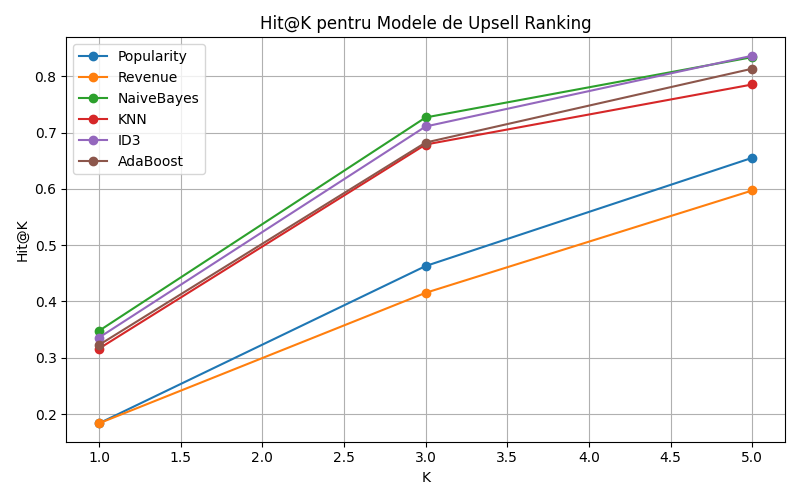
\includegraphics[width=0.75\textwidth]{hit_at_k_curve.png}
    \caption{Evoluția metricii Hit@K pentru diferite modele de upsell ranking.}
    \label{fig:hitk_curve}
\end{figure}

\subsection{Concluzii}

Rezultatele experimentale arată că modelele care folosesc informația din coș și context depășesc semnificativ metodele de tip baseline. Dintre algoritmii testați, Naive Bayes, ID3 și AdaBoost obțin cele mai bune rezultate, demonstrând că relațiile dintre produse pot fi exploatate eficient chiar și cu modele relativ simple.

De asemenea, includerea contextului temporal aduce un câștig constant de performanță, chiar dacă acesta nu este foarte mare. Acest lucru sugerează că momentul achiziției influențează comportamentul de cumpărare.


\subsection{Direcții de îmbunătățire}
O direcție de îmbunătățire ar putea fi includerea unor informații suplimentare disponibile în date, cum ar fi cantitatea achiziționată din fiecare produs sau frecvența cu care anumite produse apar în același coș.
În acest fel, am putea diferenția mai clar produsele în funție de relevanță.

În plus, dacă datele ar permite, am putea utiliza un istoric al comportamentului de cumpărare al clientului, care ar putea conduce la recomandări mai bine adaptate preferințelor acestuia.


\end{document}